\documentclass[10pt,a4paper]{article}

% -----------------------------------------------------------------------------
% MATHS MANTHAN | Class 10 Some Applications of Trigonometry Master Handbook
% Academic Year 2026--27 | Publication-quality LaTeX source with Vector TikZ.
% Compliant with latest rationalized CBSE curriculum (<= 2 right triangles).
% Compile with pdfLaTeX twice for full resolution of LastPage cross-references.
% -----------------------------------------------------------------------------

\usepackage[a4paper,top=12mm,bottom=16mm,left=15mm,right=15mm,footskip=8mm]{geometry}
\usepackage[T1]{fontenc}
\usepackage{lmodern}
\usepackage{microtype}
\usepackage{amsmath,amssymb}
\usepackage[table]{xcolor}
\usepackage{array,tabularx,booktabs}
\usepackage{graphicx}
\usepackage{eso-pic}
\usepackage{tikz}
\usetikzlibrary{calc,positioning,arrows.meta,shapes.geometric,patterns}
\usepackage[most]{tcolorbox}
\usepackage{enumitem}
\usepackage{fancyhdr}
\usepackage{lastpage}
\usepackage[hidelinks]{hyperref}
\usepackage{url}

% ============================================================================
% BRAND COLOR PALETTE — MATCHED TO THE MATHS MANTHAN STANDARD
% Primary navy: #001F49 | Brand gold: #D19029
% ============================================================================
\definecolor{primary}{RGB}{0,31,73}
\definecolor{brandnavy}{RGB}{0,31,73}
\definecolor{accent}{RGB}{209,144,41}
\definecolor{brandgold}{RGB}{209,144,41}
\definecolor{secondary}{RGB}{75,85,99}
\definecolor{lightgray}{RGB}{246,248,250}
\definecolor{accentlight}{RGB}{254,250,242}
\definecolor{primarylight}{RGB}{240,244,250}

\colorlet{navy}{primary}
\colorlet{blue}{primary!82!black}
\colorlet{gold}{accent}
\colorlet{goldpale}{accentlight}
\colorlet{bluepale}{primarylight}
\colorlet{ink}{secondary}
\colorlet{muted}{secondary}
\colorlet{linegray}{primary!25}
\colorlet{reddeep}{primary}
\colorlet{redpale}{lightgray}
\colorlet{green}{primary}
\colorlet{greenpale}{primarylight}

% -----------------------------------------------------------------------------
% ROBUST LOGO DISCOVERY (TeXworks / pdfLaTeX)
% -----------------------------------------------------------------------------
\graphicspath{{./}}
\newif\ifMMLogoFound
\MMLogoFoundfalse
\def\MMLogoFile{mathsmanthan_logo.png}
\IfFileExists{mathsmanthan_logo.png}{%
  \MMLogoFoundtrue
}{%
  \IfFileExists{mathsmanthan logo.png}{%
    \def\MMLogoFile{mathsmanthan logo.png}%
    \MMLogoFoundtrue
  }{%
    \PackageWarningNoLine{MathsManthan}{Logo image not found. Put mathsmanthan_logo.png in the same folder as this .tex file}%
  }%
}

% Automatic low-opacity logo watermark on every page
\ifMMLogoFound
  \AddToShipoutPictureBG{%
    \begin{tikzpicture}[remember picture,overlay]
      \node[opacity=0.065] at (current page.center) {%
        \includegraphics[width=0.55\paperwidth,keepaspectratio]{\MMLogoFile}%
      };
    \end{tikzpicture}%
  }%
\fi

\hypersetup{
  pdftitle={Class 10 Some Applications of Trigonometry | Maths Manthan Handbook},
  pdfauthor={Maths Manthan Tuition Classes},
  pdfsubject={CBSE Class 10 Mathematics, Academic Year 2026--27},
  pdfkeywords={Trigonometry, Heights and Distances, Class 10, CBSE, Maths Manthan, Formula Handbook}
}

\setlength{\parindent}{0pt}
\setlength{\parskip}{2.5pt}
\renewcommand{\arraystretch}{1.14}
\setlist[itemize]{leftmargin=5mm,itemsep=1.5pt,topsep=1.5pt,parsep=0pt}
\setlist[enumerate]{leftmargin=6mm,itemsep=1.5pt,topsep=1.5pt,parsep=0pt}
\setlength{\tabcolsep}{4.5pt}
\emergencystretch=2em
\hfuzz=1pt

% ============================================================================
% HEADER / FOOTER
% ============================================================================
\newcommand{\TuitionName}{{\color{primary}MATHS} {\color{accent}MANTHAN}}
\newcommand{\TuitionSub}{{\color{primary}\textbullet\ \ \text{TUITION CLASSES}\ \ \textbullet}}
\newcommand{\ContactInfo}{e-mail: contact@mathsmanthan.co.in \quad$\vert$\quad Helpline: +91-8171546558}
\newcommand{\HandbookFooterTitle}{Class 10 Some Applications of Trigonometry Handbook}

\pagestyle{fancy}
\fancyhf{}
\renewcommand{\headrulewidth}{0pt}
\renewcommand{\footrulewidth}{0.6pt}
\renewcommand{\footrule}{\hbox to\headwidth{\color{primary!30}\leaders\hrule height 0.6pt\hfill}}
\fancyfoot[L]{\footnotesize\href{https://mathsmanthan.co.in}{\textcolor{secondary}{\TuitionName\ $\vert$\ \HandbookFooterTitle}}}
\fancyfoot[R]{\footnotesize\textbf{\color{primary}Page \thepage\ of \pageref{LastPage}}\quad\textcolor{accent}{\textbf{Academic Year 2026--27}}}

\fancypagestyle{plain}{%
  \fancyhf{}
  \fancyfoot[L]{\footnotesize\href{https://mathsmanthan.co.in}{\textcolor{secondary}{\TuitionName\ $\vert$\ \HandbookFooterTitle}}}
  \fancyfoot[R]{\footnotesize\textbf{\color{primary}Page \thepage\ of \pageref{LastPage}}\quad\textcolor{accent}{\textbf{Academic Year 2026--27}}}
  \renewcommand{\headrulewidth}{0pt}
  \renewcommand{\footrulewidth}{0.6pt}
  \renewcommand{\footrule}{\hbox to\headwidth{\color{primary!30}\leaders\hrule height 0.6pt\hfill}}
}

% Reusable design components
\newcommand{\BrandMark}{%
  \ifMMLogoFound
    \includegraphics[width=22mm,height=22mm,keepaspectratio]{\MMLogoFile}%
  \else
    
\begin{tikzpicture}[baseline=-0.6ex]
      \fill[navy,rounded corners=2.2pt] (0,0) rectangle (1.45,1.05);
      \draw[gold,line width=1.2pt] (0.15,0.15)--(1.30,0.15);
      \node[text=white,font=\sffamily\bfseries\Large] at (0.725,0.59) {MM};
    \end{tikzpicture}%
  \fi
}

\newcommand{\chapterbanner}[4]{%
  \begin{tcolorbox}[enhanced,colback=bluepale,colframe=bluepale,boxrule=0pt,arc=2mm,
    left=4mm,right=4mm,top=2mm,bottom=2mm]
    {\footnotesize\bfseries\color{gold}CHAPTER #1\hfill\color{blue}#4}\par\vspace{0.6mm}
    {\LARGE\bfseries\color{navy}#2}\par
    {\small\color{muted}#3}
  \end{tcolorbox}\vspace{1mm}
}

\newcommand{\subhead}[1]{%
  \vspace{1mm}{\large\bfseries\color{navy}#1}\par\vspace{0.4mm}
  {\color{gold}\rule{13mm}{1.2pt}}\par\vspace{0.8mm}
}

\newtcolorbox{formulaBox}[1][]{enhanced,breakable,colback=goldpale,colframe=gold!65!black,
  boxrule=0.5pt,arc=1.5mm,left=3mm,right=3mm,top=1.8mm,bottom=1.8mm,
  before skip=2.5pt,after skip=3.5pt,#1}
\newtcolorbox{conceptBox}[1][]{enhanced,breakable,colback=bluepale,colframe=blue!25,
  boxrule=0.4pt,arc=1.5mm,left=3mm,right=3mm,top=1.8mm,bottom=1.8mm,
  before skip=2.5pt,after skip=3.5pt,#1}
\newtcolorbox{warningBox}[1][]{enhanced,breakable,colback=redpale,colframe=reddeep!45,
  boxrule=0.45pt,arc=1.5mm,left=3mm,right=3mm,top=1.8mm,bottom=1.8mm,
  before skip=2.5pt,after skip=3.5pt,#1}
\newtcolorbox{successBox}[1][]{enhanced,breakable,colback=greenpale,colframe=green!35,
  boxrule=0.45pt,arc=1.5mm,left=3mm,right=3mm,top=1.8mm,bottom=1.8mm,
  before skip=2.5pt,after skip=3.5pt,#1}

\newcommand{\CoreTag}{\tcbox[colback=greenpale,colframe=green!40,boxrule=.3pt,arc=1mm,left=1.5mm,right=1.5mm,top=.5mm,bottom=.5mm]{\scriptsize\bfseries\color{green}CORE SYLLABUS}}
\newcommand{\ExamTag}{\tcbox[colback=bluepale,colframe=blue!25,boxrule=.3pt,arc=1mm,left=1.5mm,right=1.5mm,top=.5mm,bottom=.5mm]{\scriptsize\bfseries\color{blue}EXAM STRATEGY}}
\newcommand{\TrapTag}{\tcbox[colback=redpale,colframe=reddeep!40,boxrule=.3pt,arc=1mm,left=1.5mm,right=1.5mm,top=.5mm,bottom=.5mm]{\scriptsize\bfseries\color{reddeep}TRAP ALERT}}
\newcommand{\WorkedTag}{\tcbox[colback=bluepale,colframe=blue!25,boxrule=.3pt,arc=1mm,left=1.5mm,right=1.5mm,top=.5mm,bottom=.5mm]{\scriptsize\bfseries\color{blue}WORKED MODEL}}
\newcommand{\SupportTag}{\tcbox[colback=accentlight,colframe=gold!55!black,boxrule=.3pt,arc=1mm,left=1.5mm,right=1.5mm,top=.5mm,bottom=.5mm]{\scriptsize\bfseries\color{primary}SUPPORTING SKILL}}
\newcommand{\ReferenceTag}{\tcbox[colback=bluepale,colframe=blue!25,boxrule=.3pt,arc=1mm,left=1.5mm,right=1.5mm,top=.5mm,bottom=.5mm]{\scriptsize\bfseries\color{primary}REFERENCE MATRIX}}

\begin{document}

% =============================================================================
% PAGE 1: COVER PAGE
% =============================================================================
\thispagestyle{fancy}
\vspace*{0mm}

\noindent
\makebox[0pt][l]{%
  \raisebox{-0.80cm}[0pt][0pt]{%
    \href{https://mathsmanthan.co.in}{%
      \BrandMark%
    }%
  }%
}%
\parbox{\textwidth}{%
  \centering
  \href{https://mathsmanthan.co.in}{%
    {\fontsize{23pt}{23pt}\selectfont\bfseries \TuitionName}\\[3pt]
    {\footnotesize\bfseries \TuitionSub}%
  }\\[2pt]
  {\scriptsize\color{secondary} \ContactInfo}
}

\vspace{5pt}
\noindent{\color{primary}\rule{0.72\textwidth}{1.5pt}}\hfill{\color{accent}\rule{0.26\textwidth}{1.5pt}}

\vspace{3mm}
\begin{center}
  {\large\bfseries\color{muted}CBSE CLASS 10 \;|\; MATHEMATICS}\\[3mm]
  {\fontsize{25}{29}\selectfont\bfseries\color{navy}SOME APPLICATIONS OF TRIGONOMETRY}\\[2mm]
  {\Large\color{blue}Heights \& Distances Master Concept, Formula \& Vector Geometry Handbook}\\[2.5mm]
  {\large\color{gold}\bfseries Academic Year 2026--27}
\end{center}

\vspace{2mm}
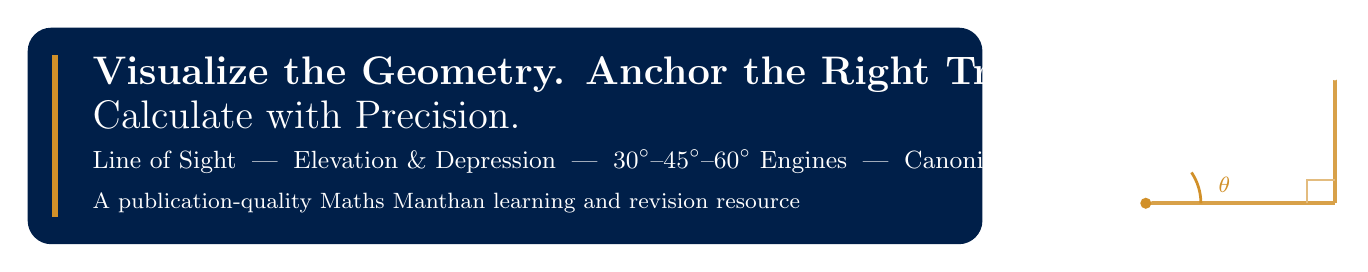
\begin{tikzpicture}
  \fill[navy,rounded corners=3mm] (0,0) rectangle (\textwidth,2.75);
  \draw[gold,line width=2pt] (0.35,0.35)--(0.35,2.40);
  \node[anchor=west,text=white,font=\bfseries\Large] at (0.7,2.15) {Visualize the Geometry. Anchor the Right Triangle.};
  \node[anchor=west,text=white,font=\Large] at (0.7,1.65) {Calculate with Precision.};
  \node[anchor=west,text=white,font=\small] at (0.7,1.05) {Line of Sight \;|\; Elevation \& Depression \;|\; 30$^\circ$--45$^\circ$--60$^\circ$ Engines \;|\; Canonical 2-Triangle Models};
  \node[anchor=west,text=white!75,font=\footnotesize] at (0.7,0.52) {A publication-quality Maths Manthan learning and revision resource};
  
  % Clinometer motif
  \draw[gold!85, line width=1.5pt] (14.2, 0.52) -- (16.6, 0.52);
  \draw[gold!85, line width=1.5pt] (16.6, 0.52) -- (16.6, 2.15);
  \draw[white, dashed, line width=1.2pt] (14.2, 0.52) -- (16.6, 2.15);
  \draw[gold, line width=1pt] (14.9, 0.52) arc (0:34:0.7);
  \node[text=gold, font=\bfseries\footnotesize] at (15.2, 0.75) {$\theta$};
  \fill[gold] (14.2, 0.52) circle (2pt);
  \fill[white] (16.6, 2.15) circle (2pt);
  \draw[gold!60, line width=0.8pt] (16.25, 0.52) -- (16.25, 0.82) -- (16.6, 0.82);
\end{tikzpicture}

\vspace{2.5mm}
\begin{minipage}[t]{0.485\textwidth}
  \begin{conceptBox}[title=What this handbook includes,fonttitle=\bfseries\color{navy}]
    \begin{itemize}
      \item Complete optical definitions: Line of Sight, Horizontal Reference Line, Observer Eye Height.
      \item Equivalence Theorem: Angle of Depression $\equiv$ Ground Elevation via alternate interior angles.
      \item The $30^\circ$--$60^\circ$--$90^\circ$ and $45^\circ$--$45^\circ$--$90^\circ$ computational scaling engines.
      \item Canonical 2-triangle models, lake reflection optics, and uniform velocity motion.
    \end{itemize}
  \end{conceptBox}
\end{minipage}\hfill
\begin{minipage}[t]{0.485\textwidth}
  \begin{formulaBox}[title=How to use it for maximum marks,fonttitle=\bfseries\color{navy}]
    \raggedright Always sketch a neat, labeled right-angled triangle diagram first (CBSE reserves 1 to 1.5 marks for the diagram alone). Explicitly declare the right triangle in text (``In right $\triangle ABC$, $\angle B = 90^\circ$''). State the ratio symbolically before substituting values. Retain surds ($\sqrt{3}, \sqrt{2}$) in factored form throughout algebraic steps; substitute decimals only on the final line if requested.
  \end{formulaBox}
\end{minipage}

\vspace{1.5mm}
\begin{warningBox}[title=Official syllabus scope (CBSE Class X 2026--27),fonttitle=\bfseries\color{navy}]
  The published CBSE Class X curriculum for 2026--27 prescribes \textbf{Heights and Distances: Angle of elevation, Angle of Depression, simple problems on heights and distances}. \\
  \textbf{Strict Constraints:} Problems should not involve more than \textbf{two right triangles}. Angles of elevation/depression are restricted exclusively to $\mathbf{30^\circ, 45^\circ, 60^\circ}$. \\
  \textbf{Excluded Topics:} 3D non-coplanar multi-plane systems, arbitrary non-standard angle tables ($15^\circ, 75^\circ$), networks with $\ge 3$ right triangles, and deleted complementary angle identities ($\tan(90^\circ-\theta)=\cot\theta$).\par
  {\scriptsize Source: \href{https://cbseacademic.nic.in/web_material/CurriculumMain27/SecPart1/Maths_SecP1X_2026-27.pdf}{CBSE Mathematics Class X Curriculum (2026--27), Unit V: Trigonometry}.}
\end{warningBox}

\vfill
\begin{center}
  {\small\bfseries\color{navy}Maths Manthan Tuition Classes}\\
  {\footnotesize\color{muted}contact@mathsmanthan.co.in \quad\textbar\quad +91-8171546558}\\
  {\footnotesize\url{https://mathsmanthan.co.in}}\\[2mm]
  {\scriptsize\color{muted}Prepared for learning and revision \;--\; not an official CBSE publication.}
\end{center}

\newpage

% =============================================================================
% PAGE 2: GEOMETRIC FOUNDATIONS OF OBSERVATION
% =============================================================================
\thispagestyle{fancy}
\vspace*{0mm}

\chapterbanner{9}{GEOMETRIC FOUNDATIONS}{The Optics of Observation: Sight Lines, Elevation \& Depression}{\CoreTag}

\subhead{Module 1 $\vert$ Core Definitions \& Physical Principles}

Trigonometric heights and distances translate surveyor and eye observations into solvable Euclidean right-angled triangles.

\begin{itemize}
  \item \textbf{Line of Sight:} The straight direct line drawn from the eye of the observer to the object viewed.
  \item \textbf{Horizontal Reference Line:} The straight horizontal line passing through the observer's eye, parallel to the ground surface.
  \item \textbf{Angle of Elevation ($\theta$):} The angle formed by the line of sight with the horizontal reference line when the target object is \textbf{above} the horizontal eye level (i.e., looking \textbf{upward}). Domain: $0^\circ < \theta < 90^\circ$.
  \item \textbf{Angle of Depression ($\phi$):} The angle formed by the line of sight with the horizontal reference line when the target object is \textbf{below} the horizontal eye level (i.e., looking \textbf{downward}). Domain: $0^\circ < \phi < 90^\circ$.
\end{itemize}

\vspace{0.8mm}
\begin{center}
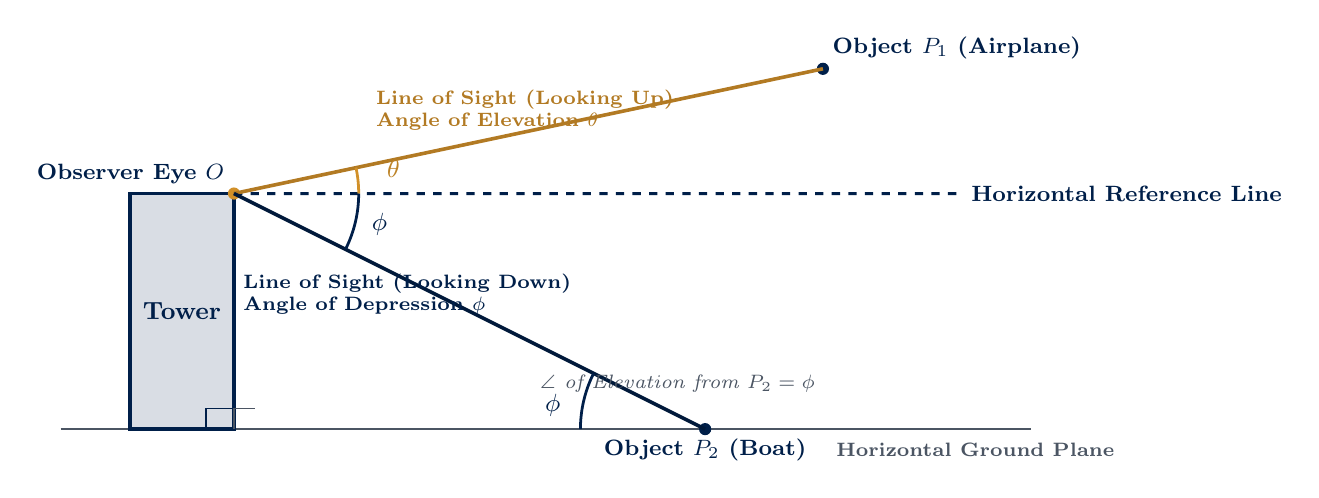
\begin{tikzpicture}[scale=0.88, >=Stealth]
  % Ground line
  \draw[thick, secondary] (-0.5, 0) -- (13.5, 0);
  \node[secondary, font=\scriptsize\bfseries] at (12.7, -0.3) {Horizontal Ground Plane};

  % Tower / Cliff
  \fill[primary!15] (0.5, 0) rectangle (2.0, 3.4);
  \draw[navy, line width=1.2pt] (0.5, 0) rectangle (2.0, 3.4);
  \node[navy, font=\bfseries\small] at (1.25, 1.7) {Tower};
  \draw[navy, line width=0.6pt] (1.6, 0) -- (1.6, 0.3) -- (2.0, 0.3);

  % Observer eye at top of tower
  \coordinate (O) at (2.0, 3.4);
  \fill[gold] (O) circle (2.5pt);
  \node[above left, navy, font=\bfseries\footnotesize] at (O) {Observer Eye $O$};

  % Horizontal line of sight from eye
  \draw[navy, dashed, line width=1.1pt] (O) -- (12.5, 3.4) coordinate (H);
  \node[right, navy, font=\bfseries\footnotesize] at (H) {Horizontal Reference Line};

  % Airplane above (Elevation)
  \coordinate (Plane) at (10.5, 5.2);
  \fill[navy] (Plane) circle (2.5pt);
  \node[above right, navy, font=\bfseries\footnotesize] at (Plane) {Object $P_1$ (Airplane)};
  \draw[gold!85!black, line width=1.3pt] (O) -- (Plane);
  \draw[gold, line width=1pt] (3.8, 3.4) arc (0:12:1.8);
  \node[gold!90!black, font=\bfseries\small] at (4.3, 3.75) {$\theta$};
  \node[gold!85!black, font=\scriptsize\bfseries, align=left] at (6.2, 4.6) {Line of Sight (Looking Up)\\\textbf{Angle of Elevation} $\theta$};

  % Boat below (Depression)
  \coordinate (Boat) at (8.8, 0);
  \fill[navy] (Boat) circle (2.5pt);
  \node[below, navy, font=\bfseries\footnotesize] at (Boat) {Object $P_2$ (Boat)};
  \draw[primary!80!black, line width=1.3pt] (O) -- (Boat);
  \draw[navy, line width=1pt] (3.8, 3.4) arc (0:-26.5:1.8);
  \node[navy, font=\bfseries\small] at (4.1, 2.95) {$\phi$};
  \node[navy, font=\scriptsize\bfseries, align=left] at (4.5, 1.95) {Line of Sight (Looking Down)\\\textbf{Angle of Depression} $\phi$};

  % Alternate interior angle at boat
  \draw[navy, line width=1pt] (7.0, 0) arc (180:153.5:1.8);
  \node[navy, font=\bfseries\small] at (6.6, 0.35) {$\phi$};
  \node[secondary, font=\scriptsize\itshape] at (8.4, 0.65) {$\angle$ of Elevation from $P_2 = \phi$};

  % Right angle at base
  \draw[secondary, line width=0.6pt] (2.0, 0) -- (2.0, 0.3) -- (2.3, 0.3);
\end{tikzpicture}
\end{center}

\vspace{-1.5mm}
\subhead{Module 2 $\vert$ The Alternate Interior Angle Theorem ($Z$-Property)}

\begin{conceptBox}[title=Mathematical Equivalence of Depression and Ground Elevation,fonttitle=\bfseries\color{navy}]
  Since the observer's horizontal reference line is mathematically parallel to the horizontal ground plane:
  $$\mathbf{\text{Horizontal Line through Eye}} \parallel \mathbf{\text{Horizontal Ground Plane}}$$
  The line of sight acts as a transversal line cutting two parallel lines. By Euclid's Alternate Interior Angles Theorem:
  $$\mathbf{\text{Angle of Depression } (\phi) = \text{Ground Angle of Elevation } (\phi)}$$
  \textbf{Operational Board Exam Rule:} When an angle of depression is stated, ALWAYS draw the dashed horizontal eye line first, mark $\phi$, and then immediately transfer $\phi$ to the ground right-angled triangle.
\end{conceptBox}

\vspace{0.5mm}
\begin{formulaBox}[title=Maths Manthan 3-Step Diagramming Protocol for Board Exams,fonttitle=\bfseries\color{navy}]
  \begin{enumerate}
    \item \textbf{Perpendicular Anchor:} Draw the ground line and vertical objects with a right-angle ($90^\circ$) symbol.
    \item \textbf{Reference Sight Line:} For depression problems, sketch the horizontal line of sight before drawing the sight ray.
    \item \textbf{Explicit Naming:} Label every vertex ($A, B, C\dots$) and declare right triangles explicitly in your working.
  \end{enumerate}
\end{formulaBox}

\newpage

% =============================================================================
% PAGE 3: OBSERVER MODELING & EYE-LEVEL SHIFT
% =============================================================================
\thispagestyle{fancy}
\vspace*{0mm}

\chapterbanner{9}{OBSERVER MODELING}{Point Observer vs. Observer with Height \& Eye-Level Mechanics}{\CoreTag}

\subhead{Module 1 $\vert$ The Geometry of Observer Height}

CBSE problems categorize observers into two distinct geometrical models:

\begin{center}
\noindent
\begin{minipage}[t]{0.485\textwidth}
  \begin{tcolorbox}[colback=bluepale,colframe=primary,boxrule=.6pt,arc=1.5mm,left=2mm,right=2mm,top=2mm,bottom=2mm]
    \centering\textbf{\color{navy}Model A: Point Observer (Height Ignored)}\par\vspace{1mm}
    \raggedright\scriptsize
    When the observer's physical height is not stated in the problem statement, the observer's eye is treated as a geometric point directly on the ground surface ($h_{\text{obs}} = 0$).
    \begin{center}
      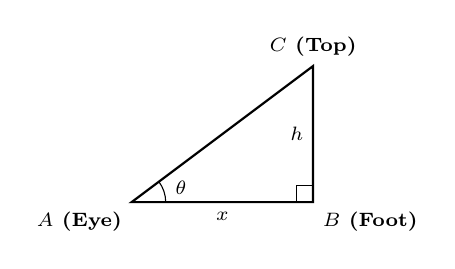
\begin{tikzpicture}[scale=0.72]
        \draw[thick] (0,0) -- (3.2,0) -- (3.2,2.4) -- cycle;
        \draw (2.9,0) rectangle (3.2,0.3);
        \node[below left, font=\scriptsize\bfseries] at (0,0) {$A$ (Eye)};
        \node[below right, font=\scriptsize\bfseries] at (3.2,0) {$B$ (Foot)};
        \node[above, font=\scriptsize\bfseries] at (3.2,2.4) {$C$ (Top)};
        \node[left, font=\scriptsize] at (3.2,1.2) {$h$};
        \node[below, font=\scriptsize] at (1.6,0) {$x$};
        \draw (0.6,0) arc (0:36.8:0.6);
        \node[right, font=\scriptsize\bfseries] at (0.6,0.25) {$\theta$};
      \end{tikzpicture}
    \end{center}
    Total Object Height: $\mathbf{h = x\tan\theta}$.
  \end{tcolorbox}
\end{minipage}\hfill
\begin{minipage}[t]{0.485\textwidth}
  \begin{tcolorbox}[colback=goldpale,colframe=gold!70!black,boxrule=.6pt,arc=1.5mm,left=2mm,right=2mm,top=2mm,bottom=2mm]
    \centering\textbf{\color{navy}Model B: Physical Observer with Height $h_{\text{obs}}$}\par\vspace{1mm}
    \raggedright\scriptsize
    When observer height is given (e.g., $1.5\,\text{m}$ tall boy), the right triangle sits on a rectangle of height $h_{\text{obs}}$. The vertical leg of the triangle is the effective height $y$.
    \begin{center}
      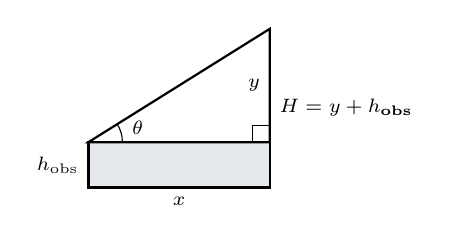
\begin{tikzpicture}[scale=0.72]
        \draw[thick, fill=primary!10] (0,0) rectangle (3.2,0.8);
        \draw[thick] (0,0.8) -- (3.2,0.8) -- (3.2,2.8) -- cycle;
        \draw (2.9,0.8) rectangle (3.2,1.1);
        \node[left, font=\scriptsize] at (0,0.4) {$h_{\text{obs}}$};
        \node[left, font=\scriptsize] at (3.2,1.8) {$y$};
        \node[right, font=\scriptsize\bfseries] at (3.2,1.4) {$H = y + h_{\text{obs}}$};
        \node[below, font=\scriptsize] at (1.6,0) {$x$};
        \draw (0.6,0.8) arc (0:32:0.6);
        \node[right, font=\scriptsize\bfseries] at (0.6,1.05) {$\theta$};
      \end{tikzpicture}
    \end{center}
    Total Height: $\mathbf{H = y + h_{\text{obs}} = x\tan\theta + h_{\text{obs}}}$.
  \end{tcolorbox}
\end{minipage}
\end{center}

\vspace{0.8mm}
\subhead{Module 2 $\vert$ Effective Vertical Leg Formulation}

\begin{formulaBox}[title=Effective Height Shift Formula,fonttitle=\bfseries\color{navy}]
  Let $H$ be the total height of a vertical tower, and $h_{\text{obs}}$ be the height of the observer.
  $$\mathbf{h_{\text{eff}} = H - h_{\text{obs}} = x\tan\theta \iff H = x\tan\theta + h_{\text{obs}}}$$
  \textbf{Critical Warning:} The right-angled triangle only models the space above the observer's eye line. Always add $h_{\text{obs}}$ back to determine the final height of the building or chimney!
\end{formulaBox}

\vspace{0.8mm}
\subhead{Module 3 $\vert$ Worked Board Archetype: The 1.5-Meter Observer}

\begin{conceptBox}[title=Standard Board Problem: Observer Viewing a Chimney,fonttitle=\bfseries\color{navy}]
  \textbf{Problem:} An observer $1.5\,\text{m}$ tall is $28.5\,\text{m}$ away from a chimney. The angle of elevation of the top of the chimney from her eyes is $45^\circ$. What is the height of the chimney? \\
  \textbf{Solution:}\par
  \textbf{Step 1: Set up the geometric model.} Let $AB$ be the chimney of total height $H$, and $CD = 1.5\,\text{m}$ be the observer. Draw horizontal line $DE \parallel CB$ meeting $AB$ at $E$. \\
  Then, $EB = CD = 1.5\,\text{m}$, and $DE = CB = 28.5\,\text{m}$. In right $\triangle ADE$, $\angle AED = 90^\circ$ and $\angle ADE = 45^\circ$. \\
  \textbf{Step 2: Calculate effective triangle height $AE$.}
  $$\tan 45^\circ = \frac{AE}{DE} \implies 1 = \frac{AE}{28.5} \implies AE = 28.5\,\text{m}$$
  \textbf{Step 3: Calculate total chimney height $H$.}
  $$H = AB = AE + EB = 28.5\,\text{m} + 1.5\,\text{m} = \mathbf{30\,\text{m}}$$
  \textbf{Final Statement:} The total height of the chimney is $\mathbf{30\,\text{m}}$.
\end{conceptBox}

\newpage

% =============================================================================
% PAGE 4: THE COMPUTATIONAL ENGINE
% =============================================================================
\thispagestyle{fancy}
\vspace*{0mm}

\chapterbanner{9}{THE COMPUTATIONAL ENGINE}{Trigonometric Ratio Selection, Exact Surds \& Geometric Scaling}{\CoreTag}

\subhead{Module 1 $\vert$ The Ratio Selection Protocol: Deciding Between $\tan$, $\sin$, and $\cos$}

\begin{center}
{\small
\begin{tabularx}{\textwidth}{@{}lcXl@{}}
  \toprule
  \textbf{\color{navy}Trig Ratio} & \textbf{\color{navy}Formula} & \textbf{\color{navy}Typical Geometric Context} & \textbf{\color{navy}Board Frequency} \\
  \midrule
  \textbf{Tangent ($\tan \theta$)} & $\dfrac{\text{Opposite}}{\text{Adjacent}} = \dfrac{h}{x}$ & Towers, buildings, statues, shadows, horizontal ground separations. & \textbf{$\approx$ 85\% of Exam Problems} \\
  \addlinespace[1pt]
  \textbf{Sine ($\sin \theta$)} & $\dfrac{\text{Opposite}}{\text{Hypotenuse}} = \dfrac{h}{L}$ & Flying kites (taut string length), broken tree trunk bent to ground, ramps. & \textbf{$\approx$ 12\% of Exam Problems} \\
  \addlinespace[1pt]
  \textbf{Cosine ($\cos \theta$)} & $\dfrac{\text{Adjacent}}{\text{Hypotenuse}} = \dfrac{x}{L}$ & Foot distance of leaning ladder from wall given physical ladder length. & \textbf{$\approx$ 3\% of Exam Problems} \\
  \bottomrule
\end{tabularx}}
\end{center}

\vspace{0.5mm}
\subhead{Module 2 $\vert$ Exact Standard Trigonometric Ratios Table for Heights \& Distances}

Under the CBSE 2026--27 curriculum, only three special acute angles are permitted:

\begin{center}
{\small
\begin{tabularx}{\textwidth}{@{}cccccX@{}}
  \toprule
  \textbf{\color{navy}Angle $\theta$} & \textbf{\color{navy}$\sin \theta$} & \textbf{\color{navy}$\cos \theta$} & \textbf{\color{navy}$\tan \theta$} & \textbf{\color{navy}$\cot \theta$} & \textbf{\color{navy}Geometric Interpretation} \\
  \midrule
  $\mathbf{30^\circ}$ & $\dfrac{1}{2}$ & $\dfrac{\sqrt{3}}{2}$ & $\mathbf{\dfrac{1}{\sqrt{3}} = \dfrac{\sqrt{3}}{3}}$ & $\mathbf{\sqrt{3}}$ & Base is $\sqrt{3} \approx 1.732$ times Height ($\text{Base} > \text{Height}$) \\
  \addlinespace[1.5pt]
  $\mathbf{45^\circ}$ & $\dfrac{1}{\sqrt{2}} = \dfrac{\sqrt{2}}{2}$ & $\dfrac{1}{\sqrt{2}} = \dfrac{\sqrt{2}}{2}$ & $\mathbf{1}$ & $\mathbf{1}$ & Isosceles Right Triangle: $\mathbf{\text{Height} = \text{Base}}$ \\
  \addlinespace[1.5pt]
  $\mathbf{60^\circ}$ & $\dfrac{\sqrt{3}}{2}$ & $\dfrac{1}{2}$ & $\mathbf{\sqrt{3}}$ & $\mathbf{\dfrac{1}{\sqrt{3}} = \dfrac{\sqrt{3}}{3}}$ & Height is $\sqrt{3} \approx 1.732$ times Base ($\text{Height} > \text{Base}$) \\
  \bottomrule
\end{tabularx}}
\end{center}

\vspace{0.5mm}
\subhead{Module 3 $\vert$ The Special Right Triangles \& Rapid Scaling Laws}

\begin{center}
\begin{minipage}[t]{0.485\textwidth}
  \begin{tcolorbox}[colback=bluepale,colframe=primary!30,boxrule=0.5pt,arc=1.5mm,left=1.5mm,right=1.5mm,top=1mm,bottom=1mm]
    \centering\textbf{\color{navy}The $45^\circ$--$45^\circ$--$90^\circ$ Triangle (Isosceles)}\par\vspace{0.3mm}
    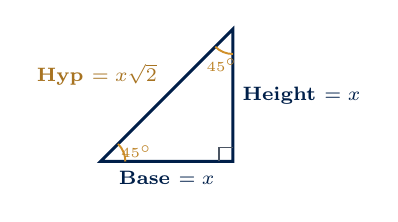
\begin{tikzpicture}[scale=0.70]
      \draw[primary, line width=1.1pt] (0,0) -- (2.4,0) -- (2.4,2.4) -- cycle;
      \draw[secondary, line width=0.4pt] (2.15,0) -- (2.15,0.25) -- (2.4,0.25);
      \draw[gold, line width=0.7pt] (0.45,0) arc (0:45:0.45);
      \node[gold!90!black, font=\bfseries\tiny] at (0.65,0.18) {$45^\circ$};
      \draw[gold, line width=0.7pt] (2.4,1.95) arc (270:225:0.45);
      \node[gold!90!black, font=\bfseries\tiny] at (2.2,1.75) {$45^\circ$};
      \node[below, navy, font=\bfseries\scriptsize] at (1.2,0) {Base $= x$};
      \node[right, navy, font=\bfseries\scriptsize] at (2.4,1.2) {Height $= x$};
      \node[above left, gold!80!black, font=\bfseries\scriptsize] at (1.2,1.2) {Hyp $= x\sqrt{2}$};
    \end{tikzpicture}\par\vspace{0.3mm}
    \textbf{Side Ratio:} $1 : 1 : \sqrt{2}$. Instant Rule: $\mathbf{\text{Height} = \text{Base}}$.
  \end{tcolorbox}
\end{minipage}\hfill
\begin{minipage}[t]{0.485\textwidth}
  \begin{tcolorbox}[colback=goldpale,colframe=gold!55!black,boxrule=0.5pt,arc=1.5mm,left=1.5mm,right=1.5mm,top=1mm,bottom=1mm]
    \centering\textbf{\color{navy}The $30^\circ$--$60^\circ$--$90^\circ$ Triangle (Scalene)}\par\vspace{0.3mm}
    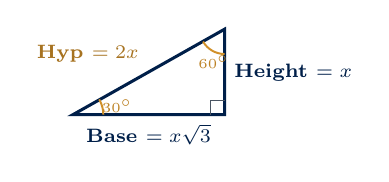
\begin{tikzpicture}[scale=0.70]
      \draw[primary, line width=1.1pt] (0,0) -- (2.75,0) -- (2.75,1.55) -- cycle;
      \draw[secondary, line width=0.4pt] (2.5,0) -- (2.5,0.25) -- (2.75,0.25);
      \draw[gold, line width=0.7pt] (0.55,0) arc (0:30:0.55);
      \node[gold!90!black, font=\bfseries\tiny] at (0.8,0.15) {$30^\circ$};
      \draw[gold, line width=0.7pt] (2.75,1.1) arc (270:210:0.45);
      \node[gold!90!black, font=\bfseries\tiny] at (2.55,0.95) {$60^\circ$};
      \node[below, navy, font=\bfseries\scriptsize] at (1.37,0) {Base $= x\sqrt{3}$};
      \node[right, navy, font=\bfseries\scriptsize] at (2.75,0.77) {Height $= x$};
      \node[above left, gold!80!black, font=\bfseries\scriptsize] at (1.37,0.77) {Hyp $= 2x$};
    \end{tikzpicture}\par\vspace{0.3mm}
    \textbf{Side Ratio:} $1 : \sqrt{3} : 2$. Opposite $30^\circ$ is half hypotenuse.
  \end{tcolorbox}
\end{minipage}
\end{center}

\vspace{0.3mm}
\subhead{Module 4 $\vert$ Essential Algebraic Surd Tools \& Rationalization}

\begin{formulaBox}[title=Golden Surd Identities for Error-Free Simplification,fonttitle=\bfseries\color{navy}]
  Never leave radicals in denominators:
  $\mathbf{\frac{1}{\sqrt{3}} = \frac{\sqrt{3}}{3}}, \quad \mathbf{\frac{1}{\sqrt{3} - 1} = \frac{\sqrt{3} + 1}{2}}, \quad \mathbf{\frac{1}{\sqrt{3} + 1} = \frac{\sqrt{3} - 1}{2}}$. \\
  \textbf{Constants:} $\sqrt{3} \approx 1.732$, $\sqrt{2} \approx 1.414$. Keep expressions factored throughout algebra; substitute decimals only on final step.
\end{formulaBox}

\newpage

% =============================================================================
% PAGE 5: SINGLE RIGHT TRIANGLE MASTER ARCHETYPES
% =============================================================================
\thispagestyle{fancy}
\vspace*{0mm}

\chapterbanner{9}{SINGLE-TRIANGLE ARCHETYPES}{Broken Tree Stem, Inclined Kite String \& Observer Models}{\WorkedTag}

\subhead{Archetype 1 $\vert$ The Broken Tree Model (Hypotenuse Fold-Over)}

\begin{minipage}[t]{0.48\textwidth}
  \textbf{Pedagogical Insight:} A tree of original vertical height $H$ breaks at point $A$ at height $y$ above the ground. The upper broken stem of length $z$ bends without detaching, touching the ground at point $C$ at distance $x$ from base $B$, forming angle $\theta$.
  \begin{itemize}
    \item Unbroken trunk: $AB = y$.
    \item Broken folded stem: $AC = z$.
    \item Ground distance: $BC = x$.
    \item Total original height: $\mathbf{H = y + z}$.
  \end{itemize}
\end{minipage}\hfill
\begin{minipage}[t]{0.48\textwidth}
  \begin{center}
  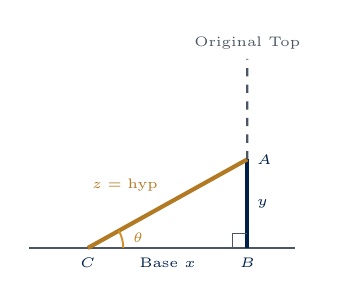
\begin{tikzpicture}[scale=0.75]
    \draw[thick, secondary] (-0.5, 0) -- (4.0, 0);
    \draw[navy, line width=1.5pt] (3.2, 0) coordinate (B) -- (3.2, 1.5) coordinate (A);
    \draw[gold!85!black, line width=1.5pt] (A) -- (0.5, 0) coordinate (C);
    \draw[secondary, dashed, line width=0.8pt] (A) -- (3.2, 3.2) coordinate (Top);
    \node[above, secondary, font=\tiny] at (Top) {Original Top};
    \draw[secondary, line width=0.4pt] (2.95, 0) -- (2.95, 0.25) -- (3.2, 0.25);
    \draw[gold, line width=0.7pt] (1.1, 0) arc (0:29:0.6);
    \node[gold!90!black, font=\bfseries\tiny] at (1.35, 0.18) {$\theta$};
    \node[below, navy, font=\bfseries\tiny] at (B) {$B$};
    \node[right, navy, font=\bfseries\tiny] at (A) {$A$};
    \node[below, navy, font=\bfseries\tiny] at (C) {$C$};
    \node[right, navy, font=\tiny] at (3.2, 0.75) {$y$};
    \node[above left, gold!85!black, font=\tiny] at (1.85, 0.8) {$z = \text{hyp}$};
    \node[below, navy, font=\tiny] at (1.85, 0) {Base $x$};
  \end{tikzpicture}
  \end{center}
\end{minipage}

\vspace{0.5mm}
\begin{formulaBox}[title=Governing Formulas \& Worked Board Archetype (8m Tree),fonttitle=\bfseries\color{navy}]
  $$\tan \theta = \frac{y}{x} \implies y = x\tan\theta, \qquad \cos \theta = \frac{x}{z} \implies z = \frac{x}{\cos\theta} \implies \mathbf{H = y + z = x\left(\frac{\sin\theta + 1}{\cos\theta}\right)}$$
  \textbf{Problem ($x = 8\,\text{m}, \theta = 30^\circ$):}
  $y = 8\tan 30^\circ = \frac{8}{\sqrt{3}}\,\text{m}, \quad z = \frac{8}{\cos 30^\circ} = \frac{16}{\sqrt{3}}\,\text{m} \implies H = \frac{24}{\sqrt{3}} = \mathbf{8\sqrt{3}\,\text{m}} \approx \mathbf{13.86\,\text{m}}$.
\end{formulaBox}

\vspace{0.8mm}
\subhead{Archetype 2 $\vert$ The Flying Kite with Incline \& Taut String}

\begin{minipage}[t]{0.52\textwidth}
  \textbf{Pedagogical Insight:} A kite flies at a vertical altitude $H$ attached to a string of length $L$ inclined at angle $\theta$ to the horizontal. If held by an observer of height $h_{\text{obs}}$, the right triangle vertical opposite is $y = H - h_{\text{obs}}$.
  $$\mathbf{\sin \theta = \frac{H - h_{\text{obs}}}{L} \implies L = \frac{H - h_{\text{obs}}}{\sin\theta}}$$
  If string is anchored directly on ground ($h_{\text{obs}} = 0$): $\mathbf{L = \frac{H}{\sin\theta}}$.
\end{minipage}\hfill
\begin{minipage}[t]{0.45\textwidth}
  \begin{center}
  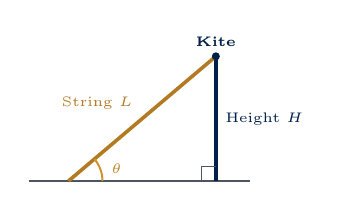
\begin{tikzpicture}[scale=0.72]
    \draw[thick, secondary] (-0.3, 0) -- (3.6, 0);
    \draw[navy, line width=1.3pt] (3.0, 0) -- (3.0, 2.2) coordinate (Kite);
    \draw[gold!85!black, line width=1.3pt] (0.4, 0) coordinate (Hand) -- (Kite);
    \fill[navy] (Kite) circle (2pt);
    \node[above, navy, font=\bfseries\tiny] at (Kite) {Kite};
    \draw[gold, line width=0.7pt] (1.0, 0) arc (0:40:0.6);
    \node[gold!90!black, font=\bfseries\tiny] at (1.25, 0.22) {$\theta$};
    \node[above left, gold!85!black, font=\tiny] at (1.7, 1.1) {String $L$};
    \node[right, navy, font=\tiny] at (3.0, 1.1) {Height $H$};
    \draw[secondary, line width=0.4pt] (2.75, 0) -- (2.75, 0.25) -- (3.0, 0.25);
  \end{tikzpicture}
  \end{center}
\end{minipage}

\vspace{0.5mm}
\begin{conceptBox}[title=Worked Board Archetype: Kite at 60m Height,fonttitle=\bfseries\color{navy}]
  \textbf{Problem:} A kite is flying at a height of $60\,\text{m}$ above the ground. The string attached is temporarily tied to a point on the ground at an inclination of $60^\circ$. Find the length of the string, assuming no slack. \\
  \textbf{Solution:} In right $\triangle ABC$, $\sin 60^\circ = \frac{60}{L} \implies \frac{\sqrt{3}}{2} = \frac{60}{L} \implies L = \frac{120}{\sqrt{3}} = \frac{120\sqrt{3}}{3} = \mathbf{40\sqrt{3}\,\text{m}} \approx \mathbf{69.28\,\text{m}}$.
\end{conceptBox}

\newpage

% =============================================================================
% PAGE 6: DUAL RIGHT TRIANGLES - NESTED SAME-SIDE ELEVATIONS
% =============================================================================
\thispagestyle{fancy}
\vspace*{0mm}

\chapterbanner{9}{DUAL-TRIANGLE GEOMETRIES}{Nested Same-Side Elevations \& Shadow Lengthening Models}{\CoreTag}

\subhead{Configuration A $\vert$ Dual Elevations on the Same Side (Moving Observer / Shadow)}

\begin{minipage}[t]{0.48\textwidth}
  \textbf{Pedagogical Principle:} An observer moves towards (or away from) a vertical tower $CD = h$ along a horizontal line. The angle of elevation changes from $\alpha$ to $\beta$ as distance $d$ is traversed. Note that as the observer moves closer, the angle strictly increases: $\mathbf{\beta > \alpha}$.
  \begin{itemize}
    \item Tower height: $CD = h$.
    \item Near ground point: $B$, with elevation $\angle CBD = \beta$.
    \item Far ground point: $A$, with elevation $\angle CAD = \alpha$.
    \item Distance traversed: $AB = d$, near distance: $BC = x$.
  \end{itemize}
\end{minipage}\hfill
\begin{minipage}[t]{0.48\textwidth}
  \begin{center}
  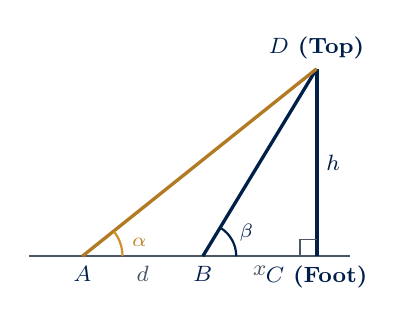
\begin{tikzpicture}[scale=0.85]
    \draw[thick, secondary] (-0.5, 0) -- (4.3, 0);
    \draw[navy, line width=1.5pt] (3.8, 0) coordinate (C) -- (3.8, 2.8) coordinate (D);
    \coordinate (B) at (2.1, 0);
    \coordinate (A) at (0.3, 0);
    \draw[navy, line width=1.2pt] (B) -- (D);
    \draw[gold!85!black, line width=1.2pt] (A) -- (D);
    \draw[secondary, line width=0.5pt] (3.55, 0) -- (3.55, 0.25) -- (3.8, 0.25);
    % Angles
    \draw[gold, line width=0.8pt] (0.9, 0) arc (0:38:0.6);
    \node[gold!90!black, font=\bfseries\scriptsize] at (1.15, 0.2) {$\alpha$};
    \draw[navy, line width=0.8pt] (2.6, 0) arc (0:58:0.5);
    \node[navy, font=\bfseries\scriptsize] at (2.75, 0.35) {$\beta$};
    % Labels
    \node[below, navy, font=\bfseries\footnotesize] at (C) {$C$ (Foot)};
    \node[above, navy, font=\bfseries\footnotesize] at (D) {$D$ (Top)};
    \node[below, navy, font=\bfseries\footnotesize] at (B) {$B$};
    \node[below, navy, font=\bfseries\footnotesize] at (A) {$A$};
    \node[right, navy, font=\footnotesize] at (3.8, 1.4) {$h$};
    \node[below, secondary, font=\footnotesize] at (1.2, 0) {$d$};
    \node[below, secondary, font=\footnotesize] at (2.95, 0) {$x$};
  \end{tikzpicture}
  \end{center}
\end{minipage}

\vspace{0.8mm}
\begin{formulaBox}[title=Master Derivation for Moving Observer / Shadow Lengthening,fonttitle=\bfseries\color{navy}]
  In right $\triangle BCD$: $\cot \beta = \dfrac{x}{h} \implies x = h\cot\beta$. \quad In right $\triangle ACD$: $\cot \alpha = \dfrac{x + d}{h} \implies x + d = h\cot\alpha$. \\
  Subtracting the first equation from the second eliminates intermediate variable $x$:
  $$\mathbf{d = h(\cot \alpha - \cot \beta) \iff h = \frac{d}{\cot \alpha - \cot \beta} = \frac{d\tan\alpha\tan\beta}{\tan\beta - \tan\alpha}}$$
  \textbf{Special Board Case ($\mathbf{\alpha = 30^\circ, \beta = 60^\circ}$):}
  $d = h\left(\sqrt{3} - \frac{1}{\sqrt{3}}\right) = h\left(\frac{2}{\sqrt{3}}\right) \implies \mathbf{h = \frac{\sqrt{3}}{2}d}, \quad \mathbf{x = \frac{d}{2}}$. \\
  \textbf{Board Strategy Tip:} Using $\cot\theta = \frac{\text{base}}{\text{height}}$ directly is faster because the unknown height $h$ remains as a common single denominator.
\end{formulaBox}

\vspace{0.5mm}
\begin{conceptBox}[title=Worked Board Archetype: Shadow Lengthening by 40 Meters,fonttitle=\bfseries\color{navy}]
  \textbf{Problem:} The shadow of a tower standing on level ground is found to be $40\,\text{m}$ longer when the Sun's altitude is $30^\circ$ than when it is $60^\circ$. Find the height of the tower. \\
  \textbf{Solution:} Let $h$ be the height of tower $CD$, and $x = BC$ be the shadow at $60^\circ$.
  $$\text{In right }\triangle BCD:\ \tan 60^\circ = \frac{h}{x} \implies \sqrt{3} = \frac{h}{x} \implies x = \frac{h}{\sqrt{3}}$$
  $$\text{In right }\triangle ACD:\ \tan 30^\circ = \frac{h}{x + 40} \implies \frac{1}{\sqrt{3}} = \frac{h}{\dfrac{h}{\sqrt{3}} + 40} \implies \frac{h}{\sqrt{3}} + 40 = h\sqrt{3}$$
  $$40 = h\sqrt{3} - \frac{h}{\sqrt{3}} = h\left(\frac{3 - 1}{\sqrt{3}}\right) = \frac{2h}{\sqrt{3}} \implies h = \frac{40\sqrt{3}}{2} = \mathbf{20\sqrt{3}\,\text{m}} \approx \mathbf{34.64\,\text{m}}$$
\end{conceptBox}

\newpage

% =============================================================================
% PAGE 7: DUAL RIGHT TRIANGLES - OPPOSITE-SIDE RIVER CROSSINGS
% =============================================================================
\thispagestyle{fancy}
\vspace*{0mm}

\chapterbanner{9}{DUAL-TRIANGLE GEOMETRIES}{Opposite-Side Observations \& River Width Models}{\CoreTag}

\subhead{Configuration B $\vert$ Observers on Opposite Sides of a Monument (River Crossing)}

\begin{minipage}[t]{0.50\textwidth}
  \textbf{Pedagogical Principle:} Two observation points $P$ and $Q$ lie on opposite sides of a central vertical tower or lighthouse $CD = h$ (e.g., opposite banks of a river or two ships on opposite sides of a light tower). The angles of elevation to the top are $\alpha$ and $\beta$.
  \begin{itemize}
    \item Monument height: $CD = h$.
    \item Distance of first point: $x_1 = PC$.
    \item Distance of second point: $x_2 = CQ$.
    \item Total separation distance: $\mathbf{W = PQ = x_1 + x_2}$.
  \end{itemize}
\end{minipage}\hfill
\begin{minipage}[t]{0.48\textwidth}
  \begin{center}
  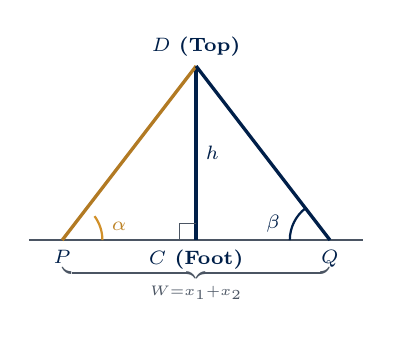
\begin{tikzpicture}[scale=0.85]
    \draw[thick, secondary] (-0.3, 0) -- (4.7, 0);
    \draw[navy, line width=1.5pt] (2.2, 0) coordinate (C) -- (2.2, 2.6) coordinate (D);
    \coordinate (P) at (0.2, 0);
    \coordinate (Q) at (4.2, 0);
    \draw[gold!85!black, line width=1.2pt] (P) -- (D);
    \draw[navy, line width=1.2pt] (Q) -- (D);
    \draw[secondary, line width=0.5pt] (1.95, 0) -- (1.95, 0.25) -- (2.2, 0.25);
    \draw[gold, line width=0.8pt] (0.8, 0) arc (0:36.5:0.6);
    \node[gold!90!black, font=\scriptsize\bfseries] at (1.05, 0.2) {$\alpha$};
    \draw[navy, line width=0.8pt] (3.6, 0) arc (180:127.5:0.6);
    \node[navy, font=\scriptsize\bfseries] at (3.35, 0.25) {$\beta$};
    \node[below, navy, font=\scriptsize\bfseries] at (P) {$P$};
    \node[below, navy, font=\scriptsize\bfseries] at (Q) {$Q$};
    \node[below, navy, font=\scriptsize\bfseries] at (C) {$C$ (Foot)};
    \node[above, navy, font=\scriptsize\bfseries] at (D) {$D$ (Top)};
    \node[right, navy, font=\scriptsize] at (2.2, 1.3) {$h$};
    \node[below, secondary, font=\scriptsize] at (2.2, -0.2) {$\underbrace{\hspace{3.4cm}}_{W = x_1 + x_2}$};
  \end{tikzpicture}
  \end{center}
\end{minipage}

\vspace{0.8mm}
\begin{formulaBox}[title=Master Governing Formula for Opposite-Side Configurations,fonttitle=\bfseries\color{navy}]
  $$\text{In right }\triangle PCD:\ \cot\alpha = \frac{x_1}{h} \implies x_1 = h\cot\alpha, \qquad \text{In right }\triangle QCD:\ \cot\beta = \frac{x_2}{h} \implies x_2 = h\cot\beta$$
  $$\mathbf{W = x_1 + x_2 = h(\cot\alpha + \cot\beta) = h\left(\frac{\tan\alpha + \tan\beta}{\tan\alpha\tan\beta}\right)}$$
  \textbf{Comparison Rule:} Same-side points \textbf{subtract} distances: $d = h(\cot\alpha - \cot\beta)$. Opposite-side points \textbf{add} distances: $W = h(\cot\alpha + \cot\beta)$.
\end{formulaBox}

\vspace{0.5mm}
\begin{conceptBox}[title=Worked Board Archetype: Two Ships on Opposite Sides of a Lighthouse,fonttitle=\bfseries\color{navy}]
  \textbf{Problem:} As observed from the top of a $75\,\text{m}$ high lighthouse from the sea-level, the angles of depression of two ships on opposite sides of the lighthouse are $30^\circ$ and $45^\circ$. Find the distance between the two ships. \\
  \textbf{Solution:}\par
  \textbf{Step 1: Declare the geometry.} Let lighthouse $CD = 75\,\text{m}$. Let $P$ and $Q$ be the two ships on opposite sides. Angles of depression equal angles of elevation $\angle DPC = 30^\circ$ and $\angle DQC = 45^\circ$ by alternate interior angles. \\
  \textbf{Step 2: Distance to ship $P$.} In right $\triangle PCD$:
  $$\tan 30^\circ = \frac{CD}{PC} \implies \frac{1}{\sqrt{3}} = \frac{75}{x_1} \implies x_1 = 75\sqrt{3}\,\text{m}$$
  \textbf{Step 3: Distance to ship $Q$.} In right $\triangle QCD$:
  $$\tan 45^\circ = \frac{CD}{QC} \implies 1 = \frac{75}{x_2} \implies x_2 = 75\,\text{m}$$
  \textbf{Step 4: Total distance $W$ between ships.}
  $$W = x_1 + x_2 = 75\sqrt{3} + 75 = \mathbf{75(\sqrt{3} + 1)\,\text{m}} \approx 75(2.732) = \mathbf{204.9\,\text{m}}$$
\end{conceptBox}

\newpage

% =============================================================================
% PAGE 8: MULTI-LEVEL SYSTEMS - PEDESTALS & STATUES
% =============================================================================
\thispagestyle{fancy}
\vspace*{0mm}

\chapterbanner{9}{MULTI-LEVEL SYSTEMS}{Pedestals, Flagstaffs \& Vertical Stacking Geometries}{\CoreTag}

\subhead{Configuration C $\vert$ Statue or Flagstaff Atop a Pedestal / Building}

\begin{minipage}[t]{0.48\textwidth}
  \textbf{Pedagogical Principle:} A statue or flagstaff of height $p$ sits atop a pedestal/building of height $h$. From a single ground observation point $D$ at distance $x$, the angles of elevation to the bottom and top of the statue are $\alpha$ and $\beta$ ($\beta > \alpha$).
  \begin{itemize}
    \item Lower pedestal: $BC = h$.
    \item Upper statue: $AB = p$. Total height: $AC = h + p$.
    \item Common horizontal base: $CD = x$.
  \end{itemize}
\end{minipage}\hfill
\begin{minipage}[t]{0.48\textwidth}
  \begin{center}
  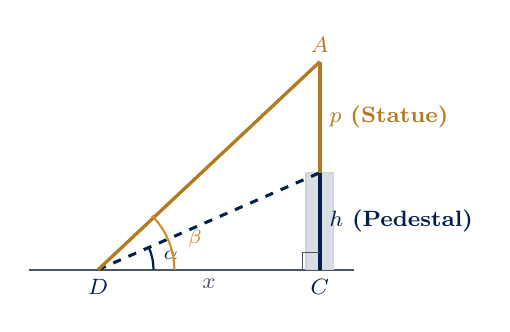
\begin{tikzpicture}[scale=0.88]
    \draw[thick, secondary] (-0.5, 0) -- (4.2, 0);
    \draw[primary!20, fill=primary!15] (3.5, 0) rectangle (3.9, 1.4);
    \draw[navy, line width=1.3pt] (3.7, 0) coordinate (C) -- (3.7, 1.4) coordinate (B);
    \draw[gold!85!black, line width=1.6pt] (3.7, 1.4) -- (3.7, 3.0) coordinate (A);
    \coordinate (D) at (0.5, 0);
    \draw[navy, dashed, line width=1.1pt] (D) -- (B);
    \draw[gold!85!black, line width=1.2pt] (D) -- (A);
    \draw[secondary, line width=0.5pt] (3.45, 0) -- (3.45, 0.25) -- (3.7, 0.25);
    % Angles
    \draw[navy, line width=0.8pt] (1.3, 0) arc (0:23.6:0.8);
    \node[navy, font=\bfseries\scriptsize] at (1.55, 0.2) {$\alpha$};
    \draw[gold, line width=0.8pt] (1.6, 0) arc (0:45:1.1);
    \node[gold!90!black, font=\bfseries\scriptsize] at (1.9, 0.45) {$\beta$};
    % Labels
    \node[below, navy, font=\bfseries\footnotesize] at (D) {$D$};
    \node[below, navy, font=\bfseries\footnotesize] at (C) {$C$};
    \node[right, navy, font=\bfseries\footnotesize] at (3.7, 0.7) {$h$ (Pedestal)};
    \node[right, gold!85!black, font=\bfseries\footnotesize] at (3.7, 2.2) {$p$ (Statue)};
    \node[above, gold!85!black, font=\bfseries\footnotesize] at (A) {$A$};
    \node[below, secondary, font=\footnotesize] at (2.1, 0) {$x$};
  \end{tikzpicture}
  \end{center}
\end{minipage}

\vspace{0.8mm}
\begin{formulaBox}[title=Master Governing Formulas for Pedestal \& Statue,fonttitle=\bfseries\color{navy}]
  $$\text{In }\triangle BCD:\ x = \frac{h}{\tan\alpha} = h\cot\alpha. \qquad \text{In }\triangle ACD:\ x = \frac{h + p}{\tan\beta}$$
  Equating the common base $x$ yields the direct closed-form formulas:
  $$\mathbf{p = x(\tan\beta - \tan\alpha) = h\left(\frac{\tan\beta}{\tan\alpha} - 1\right) \iff h = \frac{p\tan\alpha}{\tan\beta - \tan\alpha}}$$
\end{formulaBox}

\vspace{0.5mm}
\begin{conceptBox}[title=Worked Board Archetype: Statue of Height 1.6m on Pedestal,fonttitle=\bfseries\color{navy}]
  \textbf{Problem:} A $1.6\,\text{m}$ tall statue stands on the top of a pedestal. From a point on the ground, the angle of elevation of the top of the statue is $60^\circ$ and from the same point the angle of elevation of the top of the pedestal is $45^\circ$. Find the height of the pedestal. \\
  \textbf{Solution:} Let pedestal height be $h = BC$, statue $p = AB = 1.6\,\text{m}$, and base $CD = x$.
  $$\text{In right }\triangle BCD:\ \tan 45^\circ = \frac{h}{x} \implies 1 = \frac{h}{x} \implies x = h$$
  $$\text{In right }\triangle ACD:\ \tan 60^\circ = \frac{h + 1.6}{x} \implies \sqrt{3} = \frac{h + 1.6}{h} \implies h\sqrt{3} = h + 1.6$$
  $$h(\sqrt{3} - 1) = 1.6 \implies h = \frac{1.6}{\sqrt{3} - 1} = \frac{1.6(\sqrt{3} + 1)}{3 - 1} = \mathbf{0.8(\sqrt{3} + 1)\,\text{m}} \approx 0.8(2.732) = \mathbf{2.186\,\text{m}}$$
\end{conceptBox}

\vspace{0.8mm}
\begin{warningBox}[title=Common Board Exam Pitfall on Pedestals,fonttitle=\bfseries\color{navy}]
  Students frequently make the fatal mistake of assuming $\triangle ABD$ is a right-angled triangle. It is NOT! The right angle is strictly at the ground base $C$. Always formulate equations using right $\triangle BCD$ and right $\triangle ACD$.
\end{warningBox}

\newpage

% =============================================================================
% PAGE 9: MULTI-LEVEL SYSTEMS - BUILDING TO TOWER
% =============================================================================
\thispagestyle{fancy}
\vspace*{0mm}

\chapterbanner{9}{MULTI-LEVEL SYSTEMS}{Building-to-Tower: Elevation \& Depression Combinations}{\CoreTag}

\subhead{Configuration D $\vert$ Building to Adjacent Tower (Elevation + Depression Dual)}

\begin{minipage}[t]{0.48\textwidth}
  \textbf{Pedagogical Principle:} An observer standing on top of a building of height $h$ views an adjacent taller cable tower:
  \begin{itemize}
    \item Looking \textbf{up} at the top: Angle of elevation $= \alpha$.
    \item Looking \textbf{down} at the foot: Angle of depression $= \beta$.
    \item Rectangle formed: $ABDE$ has height $h$ and width $x$.
    \item Tower height: $\mathbf{H = CD = CE + h}$.
  \end{itemize}
\end{minipage}\hfill
\begin{minipage}[t]{0.48\textwidth}
  \begin{center}
  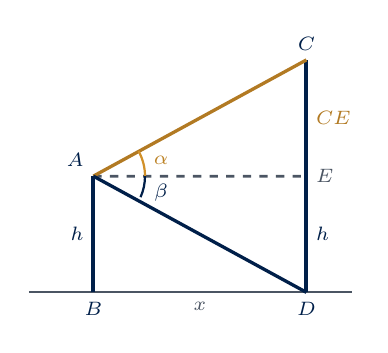
\begin{tikzpicture}[scale=0.82]
    \draw[thick, secondary] (-0.5, 0) -- (4.5, 0);
    % Building AB
    \draw[navy, line width=1.4pt] (0.5, 0) coordinate (B) -- (0.5, 1.8) coordinate (A);
    % Tower CD
    \draw[navy, line width=1.5pt] (3.8, 0) coordinate (D) -- (3.8, 3.6) coordinate (C);
    % Horizontal line of sight AE
    \draw[secondary, dashed, line width=1pt] (A) -- (3.8, 1.8) coordinate (E);
    % Lines of sight
    \draw[gold!85!black, line width=1.2pt] (A) -- (C);
    \draw[navy, line width=1.2pt] (A) -- (D);
    % Angles
    \draw[gold, line width=0.8pt] (1.3, 1.8) arc (0:29:0.8);
    \node[gold!90!black, font=\scriptsize\bfseries] at (1.55, 2.05) {$\alpha$};
    \draw[navy, line width=0.8pt] (1.3, 1.8) arc (0:-24:0.8);
    \node[navy, font=\scriptsize\bfseries] at (1.55, 1.55) {$\beta$};
    % Labels
    \node[below, navy, font=\scriptsize\bfseries] at (B) {$B$};
    \node[above left, navy, font=\scriptsize\bfseries] at (A) {$A$};
    \node[below, navy, font=\scriptsize\bfseries] at (D) {$D$};
    \node[above, navy, font=\scriptsize\bfseries] at (C) {$C$};
    \node[right, secondary, font=\scriptsize] at (E) {$E$};
    \node[left, navy, font=\scriptsize] at (0.5, 0.9) {$h$};
    \node[right, navy, font=\scriptsize] at (3.8, 0.9) {$h$};
    \node[right, gold!85!black, font=\scriptsize] at (3.8, 2.7) {$CE$};
    \node[below, secondary, font=\scriptsize] at (2.15, 0) {$x$};
  \end{tikzpicture}
  \end{center}
\end{minipage}

\vspace{0.8mm}
\begin{formulaBox}[title=Governing Formula for Building-to-Tower Observation,fonttitle=\bfseries\color{navy}]
  $$\text{In right }\triangle ADE:\ \tan\beta = \frac{DE}{AE} = \frac{h}{x} \implies x = \frac{h}{\tan\beta} = h\cot\beta$$
  $$\text{In right }\triangle ACE:\ CE = x\tan\alpha = (h\cot\beta)\tan\alpha = h\frac{\tan\alpha}{\tan\beta}$$
  $$\mathbf{H_{\text{tower}} = CD = CE + ED = h\left(1 + \frac{\tan\alpha}{\tan\beta}\right) = h(1 + \tan\alpha\cot\beta)}$$
\end{formulaBox}

\vspace{0.5mm}
\begin{conceptBox}[title=Worked Board Archetype: 7m Building and Cable Tower,fonttitle=\bfseries\color{navy}]
  \textbf{Problem:} From the top of a $7\,\text{m}$ high building, the angle of elevation of the top of a cable tower is $60^\circ$ and the angle of depression of its foot is $45^\circ$. Determine the height of the tower. \\
  \textbf{Solution:}\par
  \textbf{Step 1: Set up rectangle and right triangles.} Let $AB = 7\,\text{m}$ be the building and $CD$ be the cable tower. Draw horizontal line $AE \perp CD$. Then $AB = ED = 7\,\text{m}$ and $AE = BD = x$. \\
  \textbf{Step 2: Find width $x$ from angle of depression.} In right $\triangle ADE$:
  $$\tan 45^\circ = \frac{DE}{AE} \implies 1 = \frac{7}{x} \implies x = 7\,\text{m}$$
  \textbf{Step 3: Find upper segment $CE$ from angle of elevation.} In right $\triangle ACE$:
  $$\tan 60^\circ = \frac{CE}{AE} \implies \sqrt{3} = \frac{CE}{7} \implies CE = 7\sqrt{3}\,\text{m}$$
  \textbf{Step 4: Total height of the cable tower.}
  $$H = CD = CE + ED = 7\sqrt{3} + 7 = \mathbf{7(\sqrt{3} + 1)\,\text{m}} \approx 7(2.732) = \mathbf{19.124\,\text{m}}$$
\end{conceptBox}

\newpage

% =============================================================================
% PAGE 10: ADVANCED BOARD ARCHETYPES - LAKE REFLECTION (HOTS)
% =============================================================================
\thispagestyle{fancy}
\vspace*{0mm}

\chapterbanner{9}{ADVANCED BOARD MODELS (HOTS)}{Lake Reflection Optics: Real Cloud vs. Virtual Image}{\WorkedTag}

\subhead{HOTS Archetype 1 $\vert$ The Cloud and its Reflection in a Lake}

\begin{minipage}[t]{0.50\textwidth}
  \textbf{Optical Law in Trigonometry:} By specular reflection from a calm lake surface, the depth of the virtual image ($C'$) beneath the water level is strictly equal to the height of the real cloud ($C$) above the water level:
  $$\mathbf{\text{Cloud Height } H = \text{Virtual Image Depth } H}$$
  Let the observer be at platform height $h$ above water level.
  \begin{itemize}
    \item Real cloud altitude above observer: $CM = H - h$.
    \item Virtual image depth below observer: $C'M = H + h$.
    \item Horizontal distance to cloud: $AM = x$.
  \end{itemize}
\end{minipage}\hfill
\begin{minipage}[t]{0.48\textwidth}
  \begin{center}
  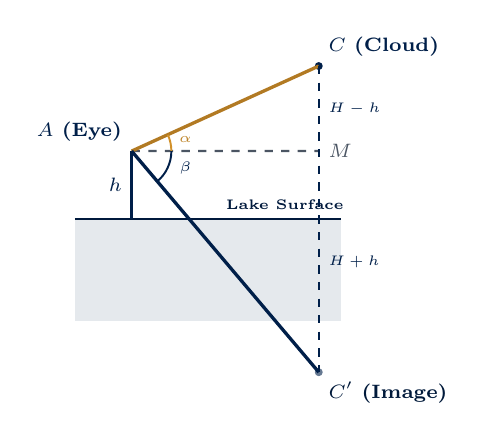
\begin{tikzpicture}[scale=0.72]
    % Water surface
    \fill[primary!10] (-0.5, -1.8) rectangle (4.2, 0);
    \draw[blue, thick] (-0.5, 0) -- (4.2, 0);
    \node[above, blue, font=\tiny\bfseries] at (3.2, 0) {Lake Surface};

    % Observer platform
    \draw[navy, line width=1.3pt] (0.5, 0) -- (0.5, 1.2) coordinate (A);
    \node[left, navy, font=\scriptsize] at (0.5, 0.6) {$h$};
    \node[above left, navy, font=\scriptsize\bfseries] at (A) {$A$ (Eye)};

    % Horizontal sightline
    \draw[secondary, dashed, line width=0.8pt] (A) -- (3.8, 1.2) coordinate (M);
    \node[right, secondary, font=\scriptsize] at (M) {$M$};

    % Real Cloud C
    \coordinate (C) at (3.8, 2.7);
    \fill[navy] (C) circle (2pt);
    \node[above right, navy, font=\scriptsize\bfseries] at (C) {$C$ (Cloud)};
    \draw[gold!85!black, line width=1.2pt] (A) -- (C);

    % Virtual Reflection C'
    \coordinate (Cprime) at (3.8, -2.7);
    \fill[primary!60] (Cprime) circle (2pt);
    \node[below right, primary!80!black, font=\scriptsize\bfseries] at (Cprime) {$C'$ (Image)};
    \draw[navy, line width=1.2pt] (A) -- (Cprime);

    % Vertical drop line
    \draw[navy, dashed, line width=0.7pt] (C) -- (Cprime);

    % Angles
    \draw[gold, line width=0.7pt] (1.2, 1.2) arc (0:24:0.7);
    \node[gold!90!black, font=\tiny\bfseries] at (1.45, 1.4) {$\alpha$};
    \draw[navy, line width=0.7pt] (1.2, 1.2) arc (0:-50:0.7);
    \node[navy, font=\tiny\bfseries] at (1.45, 0.9) {$\beta$};

    % Dimensions
    \node[right, navy, font=\tiny] at (3.8, 1.95) {$H - h$};
    \node[right, navy, font=\tiny] at (3.8, -0.75) {$H + h$};
  \end{tikzpicture}
  \end{center}
\end{minipage}

\vspace{0.8mm}
\begin{formulaBox}[title=Closed-Form Derivation for Cloud Altitude above Water,fonttitle=\bfseries\color{navy}]
  $$\text{In right }\triangle ACM:\ x = \frac{H - h}{\tan\alpha}, \qquad \text{In right }\triangle AC'M:\ x = \frac{H + h}{\tan\beta}$$
  Equating expressions for horizontal separation $x$:
  $$\frac{H - h}{\tan\alpha} = \frac{H + h}{\tan\beta} \implies (H - h)\tan\beta = (H + h)\tan\alpha \iff \mathbf{H = h\left(\frac{\tan\beta + \tan\alpha}{\tan\beta - \tan\alpha}\right)}$$
\end{formulaBox}

\vspace{0.5mm}
\begin{conceptBox}[title=Worked Board Archetype: Cloud at 60m Platform Height,fonttitle=\bfseries\color{navy}]
  \textbf{Problem:} The angle of elevation of a cloud from a point $60\,\text{m}$ above a lake is $30^\circ$ and the angle of depression of its reflection in the lake is $60^\circ$. Find the height of the cloud above the lake. \\
  \textbf{Solution:} Let $H$ be cloud height above lake, and $h = 60\,\text{m}$. In $\triangle ACM$ and $\triangle AC'M$:
  $$\tan 30^\circ = \frac{H - 60}{x} \implies x = (H - 60)\sqrt{3}, \qquad \tan 60^\circ = \frac{H + 60}{x} \implies x = \frac{H + 60}{\sqrt{3}}$$
  $$(H - 60)\sqrt{3} = \frac{H + 60}{\sqrt{3}} \implies 3(H - 60) = H + 60 \implies 2H = 240 \implies \mathbf{H = 120\,\text{m}}$$
  \textbf{Final Statement:} The height of the cloud above the lake surface is $\mathbf{120\,\text{m}}$.
\end{conceptBox}

\newpage

% =============================================================================
% PAGE 11: ADVANCED BOARD ARCHETYPES - UNIFORM VELOCITY (HOTS)
% =============================================================================
\thispagestyle{fancy}
\vspace*{0mm}

\chapterbanner{9}{ADVANCED BOARD MODELS (HOTS)}{Uniform Velocity Mechanics: Moving Aircraft \& Boats}{\WorkedTag}

\subhead{HOTS Archetype 2 $\vert$ Uniform Velocity \& Rate of Motion (Aircraft / Approaching Boat)}

\begin{minipage}[t]{0.50\textwidth}
  \textbf{Physical Principle:} An object moves along a straight horizontal path at constant speed $v$. The observation angle changes as time elapses:
  \begin{itemize}
    \item Uniform velocity equation: $\mathbf{\Delta x = v \cdot t}$.
    \item Constant altitude of airplane: $H$.
    \item Initial elevation angle at $t_1$: $\theta_1 = 60^\circ$.
    \item Final elevation angle after time $t$: $\theta_2 = 30^\circ$.
    \item Distance traversed: $\mathbf{d = x_2 - x_1}$.
    \item Uniform speed: $\mathbf{v = \frac{d}{t}}$.
  \end{itemize}
\end{minipage}\hfill
\begin{minipage}[t]{0.48\textwidth}
  \begin{center}
  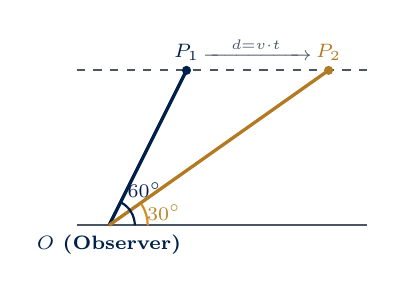
\begin{tikzpicture}[scale=0.82]
    \draw[thick, secondary] (-0.3, 0) -- (4.2, 0);
    \draw[secondary, dashed, line width=0.8pt] (-0.3, 2.4) -- (4.2, 2.4);
    \coordinate (O) at (0.2, 0);
    \coordinate (P1) at (1.4, 2.4);
    \coordinate (P2) at (3.6, 2.4);
    \draw[navy, line width=1.2pt] (O) -- (P1);
    \draw[gold!85!black, line width=1.2pt] (O) -- (P2);
    \fill[navy] (P1) circle (2pt);
    \fill[gold!85!black] (P2) circle (2pt);
    \draw[gold, line width=0.8pt] (0.8, 0) arc (0:33.3:0.6);
    \node[gold!90!black, font=\scriptsize\bfseries] at (1.05, 0.2) {$30^\circ$};
    \draw[navy, line width=0.8pt] (0.6, 0) arc (0:62.5:0.4);
    \node[navy, font=\scriptsize\bfseries] at (0.75, 0.55) {$60^\circ$};
    \node[above, navy, font=\scriptsize\bfseries] at (P1) {$P_1$};
    \node[above, gold!85!black, font=\scriptsize\bfseries] at (P2) {$P_2$};
    \node[above, secondary, font=\scriptsize] at (2.5, 2.4) {$\xrightarrow{\quad d = v\cdot t \quad}$};
    \node[below, navy, font=\scriptsize\bfseries] at (O) {$O$ (Observer)};
  \end{tikzpicture}
  \end{center}
\end{minipage}

\vspace{0.8mm}
\begin{formulaBox}[title=Governing Mathematical Derivation for Cruising Airplane,fonttitle=\bfseries\color{navy}]
  $$\text{Initial base distance: } x_1 = H\cot 60^\circ = \frac{H}{\sqrt{3}}, \qquad \text{Final base distance: } x_2 = H\cot 30^\circ = H\sqrt{3}$$
  $$\text{Horizontal distance covered in time } t:\ d = x_2 - x_1 = H\sqrt{3} - \frac{H}{\sqrt{3}} = \frac{2H}{\sqrt{3}}$$
  $$\mathbf{\text{Speed } v = \frac{d}{t} = \frac{2H}{\sqrt{3}\,t} \quad [\text{m/s}] \qquad \iff \qquad v_{\text{km/h}} = v \times \frac{18}{5} \quad [\text{km/h}]}$$
\end{formulaBox}

\vspace{0.5mm}
\begin{conceptBox}[title=Worked Board Archetype: Airplane at Altitude 1500$\sqrt{3}$ Meters,fonttitle=\bfseries\color{navy}]
  \textbf{Problem:} An aeroplane at an altitude of $1500\sqrt{3}\,\text{m}$ observes that the angle of elevation changes from $60^\circ$ to $30^\circ$ in $15$ seconds while flying horizontally. Find the speed of the aeroplane in $\text{km/h}$. \\
  \textbf{Solution:}\par
  \textbf{Step 1: Compute initial and final base distances.}
  $$x_1 = \frac{1500\sqrt{3}}{\tan 60^\circ} = \frac{1500\sqrt{3}}{\sqrt{3}} = 1500\,\text{m}, \qquad x_2 = \frac{1500\sqrt{3}}{\tan 30^\circ} = \frac{1500\sqrt{3}}{1/\sqrt{3}} = 4500\,\text{m}$$
  \textbf{Step 2: Compute distance traversed in 15 seconds.}
  $$d = x_2 - x_1 = 4500\,\text{m} - 1500\,\text{m} = 3000\,\text{m}$$
  \textbf{Step 3: Calculate speed and convert to $\text{km/h}$.}
  $$v = \frac{d}{t} = \frac{3000\,\text{m}}{15\,\text{s}} = 200\,\text{m/s} \implies \mathbf{v = 200 \times \frac{18}{5} = 40 \times 18 = 720\,\text{km/h}}$$
\end{conceptBox}

\newpage

% =============================================================================
% PAGE 12: MASTER QUICK-REVISION REFERENCE MATRIX
% =============================================================================
\thispagestyle{fancy}
\vspace*{0mm}

\chapterbanner{9}{QUICK-REVISION MATRIX}{Comprehensive Canonical Geometries \& Rapid Shortcuts}{\ReferenceTag}

\subhead{Module 1 $\vert$ Master Trigonometric Geometry Reference Matrix}

{\renewcommand{\arraystretch}{1.12}\small
\begin{tabularx}{\textwidth}{@{}lllX@{}}
  \toprule
  \textbf{\color{navy}Geometric Configuration} & \textbf{\color{navy}Primary Unknown} & \textbf{\color{navy}Governing Master Formula} & \textbf{\color{navy}10-Second Mental Check} \\
  \midrule
  \textbf{Single Triangle} & Height / Distance & $h = x\tan\theta \iff x = h\cot\theta$ & At $45^\circ$, $h = x$; at $30^\circ$, $x > h$. \\
  \addlinespace[1.5pt]
  \textbf{Broken Tree Stem} & Total Tree Height & $H = y + z = x\left(\dfrac{1 + \sin\theta}{\cos\theta}\right)$ & For $30^\circ$, $H = x\sqrt{3}$. \\
  \addlinespace[1.5pt]
  \textbf{Nested Same-Side} & Distance Traversed & $d = h(\cot\alpha - \cot\beta)$ & For $30^\circ, 60^\circ$, $h = \dfrac{\sqrt{3}}{2}d$ and $x = \dfrac{d}{2}$. \\
  \addlinespace[1.5pt]
  \textbf{Opposite-Side River} & Total Separation & $W = h(\cot\alpha + \cot\beta)$ & Always strictly greater than same-side. \\
  \addlinespace[1.5pt]
  \textbf{Statue on Pedestal} & Pedestal Height & $h = \dfrac{p\tan\alpha}{\tan\beta - \tan\alpha}$ & If $\alpha = 45^\circ, \beta = 60^\circ$, $h = \dfrac{p}{\sqrt{3}-1}$. \\
  \addlinespace[1.5pt]
  \textbf{Building to Tower} & Total Tower Height & $H = h(1 + \tan\alpha\cot\beta)$ & If $\alpha = 60^\circ, \beta = 45^\circ$, $H = h(\sqrt{3}+1)$. \\
  \addlinespace[1.5pt]
  \textbf{Cloud in Lake} & Real Cloud Height & $H = h\left(\dfrac{\tan\beta + \tan\alpha}{\tan\beta - \tan\alpha}\right)$ & If $\alpha = 30^\circ, \beta = 60^\circ$, $H = 2h$. \\
  \bottomrule
\end{tabularx}}

\vspace{1mm}
\subhead{Module 2 $\vert$ Supporting Symmetric Configuration: Two Poles of Equal Height}

\begin{conceptBox}[title=Board Model: Two Poles on Opposite Sides of an 80m Road,fonttitle=\bfseries\color{navy}]
  \textbf{Configuration:} Two poles of equal height $h$ stand on opposite sides of a road of width $W = 80\,\text{m}$. From a point between them, angles of elevation of the tops are $60^\circ$ and $30^\circ$.
  $$\tan 60^\circ = \frac{h}{x} \implies h = x\sqrt{3}, \qquad \tan 30^\circ = \frac{h}{80 - x} \implies h = \frac{80 - x}{\sqrt{3}}$$
  $$x\sqrt{3} = \frac{80 - x}{\sqrt{3}} \implies 3x = 80 - x \implies 4x = 80 \implies \mathbf{x = 20\,\text{m}}$$
  $$\mathbf{h = 20\sqrt{3}\,\text{m}}, \qquad \text{Distances from the point: } \mathbf{20\,\text{m}} \text{ and } \mathbf{60\,\text{m}}.$$
\end{conceptBox}

\vspace{0.8mm}
\subhead{Module 3 $\vert$ Classical Geometric Extension: Complementary Angles ($h = \sqrt{ab}$)}

\begin{formulaBox}[title=Complementary Observation Points Shortcut,fonttitle=\bfseries\color{navy}]
  If angles of elevation of top of a tower from two ground points at distances $a$ and $b$ from its base are \textbf{complementary} ($\alpha + \beta = 90^\circ$):
  $$\tan\alpha = \frac{h}{a}, \qquad \tan\beta = \tan(90^\circ - \alpha) = \cot\alpha = \frac{h}{b} \implies \tan\alpha \cdot \cot\alpha = \frac{h^2}{ab} = 1 \implies \mathbf{h = \sqrt{ab}}$$
\end{formulaBox}

\newpage

% =============================================================================
% PAGE 13: BOARD EXAM TRAPS & PRE-SUBMISSION AUDIT
% =============================================================================
\thispagestyle{fancy}
\vspace*{0mm}

\chapterbanner{9}{BOARD STRATEGY \& AUDIT}{Canonical Geometries, Examiner Traps \& Pre-Submission Checklist}{\ExamTag}

\subhead{Module 1 $\vert$ The Five Lethal CBSE Board Exam Traps}

\begin{warningBox}[title=Examiner Trap Alerts (Where Students Lose Marks),fonttitle=\bfseries\color{navy}]
  \begin{enumerate}
    \item \textbf{The Vertical Reference Line Blunder:} In depression problems, students often take the angle with the vertical wall. Remember: Angles of elevation and depression are \textbf{ALWAYS} measured against the horizontal reference line!
    \item \textbf{The Vanishing Observer Height:} For a $1.5\,\text{m}$ observer looking at a $30\,\text{m}$ chimney, triangle leg is $30 - 1.5 = 28.5\,\text{m}$. Forgetting to subtract initially (or forgetting to add $1.5\,\text{m}$ back at the end) loses 2 marks.
    \item \textbf{Premature Decimal Substitution:} Replacing $\sqrt{3}$ with $1.732$ early creates rounding errors. Factor common terms, simplify fractions completely, and substitute decimals only on the last line.
    \item \textbf{Missing Alternate Interior Angle Line:} When an angle of depression is given, failing to draw the horizontal line from the observer's eye is penalized under CBSE step-marking criteria.
    \item \textbf{Speed Unit Mismatch:} Calculating airplane speed as $\text{distance (meters)} / \text{time (seconds)}$ yields $\text{m/s}$. Failing to convert to $\text{km/h}$ (multiply by $18/5$) when asked costs the final accuracy mark.
  \end{enumerate}
\end{warningBox}

\vspace{0.5mm}
\subhead{Module 2 $\vert$ Rapid 15-Second Arithmetic Verification Hacks}

\begin{conceptBox}[title=Instant Mental Sanity Checks,fonttitle=\bfseries\color{navy}]
  \begin{itemize}
    \item \textbf{Distance-Angle Monotonicity:} As an observer approaches a tower, the elevation angle must strictly increase ($30^\circ \to 45^\circ \to 60^\circ$). If your calculation yields a smaller angle closer to the tower, reverse your geometry!
    \item \textbf{Isosceles Right Triangle Check:} At $45^\circ$, height must exactly equal base.
    \item \textbf{Hypotenuse Superiority:} The hypotenuse is strictly the longest side ($L > h$ and $L > x$). If string length $L$ is less than height $H$, an algebraic error has occurred.
  \end{itemize}
\end{conceptBox}

\vspace{0.5mm}
\subhead{Module 3 $\vert$ Five-Point Pre-Submission Board Exam Audit Checklist}

\begin{successBox}[title=Maths Manthan 5-Point Pre-Submission Audit Checklist,fonttitle=\bfseries\color{navy}]
  \begin{itemize}
    \item[\textbf{[ ] 1.}] \textbf{Right-Angle Symbol \& Labeled Vertices:} Is every vertical object marked perpendicular ($90^\circ$) to the ground, and are all vertices named ($A, B, C\dots$)?
    \item[\textbf{[ ] 2.}] \textbf{Triangle Declaration in Text:} Is each calculation preceded by a clear declaration (e.g., ``In right-angled triangle $ABC$, $\angle B = 90^\circ$'')?
    \item[\textbf{[ ] 3.}] \textbf{Depression Angle Construction:} Did I draw the dashed horizontal eye-line and mark alternate interior angles?
    \item[\textbf{[ ] 4.}] \textbf{Conjugate Rationalization:} Are all denominators cleared of radicals (e.g., multiplied by $\sqrt{3}+1$)?
    \item[\textbf{[ ] 5.}] \textbf{Physical Units:} Does every final answer include proper units ($\text{m}, \text{cm}, \text{km/h}$) highlighted in a neat box?
  \end{itemize}
\end{successBox}

\vfill
\begin{center}
  {\small\bfseries\color{navy}Maths Manthan Tuition Classes}\\
  {\footnotesize\color{muted}contact@mathsmanthan.co.in \quad\textbar\quad +91-8171546558 \quad\textbar\quad \url{https://mathsmanthan.co.in}}\\[1.5mm]
  {\scriptsize\color{muted}\textbf{End of Chapter 9 Handbook} \;--\; Designed for Academic Excellence in CBSE Board Examinations.}
\end{center}

\end{document}
